\section{Dialog Motor (Antriebsdaten)}
Wenn im Folgenden von Motor die Rede ist, so ist das Antriebskonzept im Loksim gemeint. Es wird immer mit den Summen aller Motoren eines Triebfahrzeuges gerechnet. Loksim kennt derzeit keine Differenzierung einzelner Motoren, Motortypen oder Triebfahrzeugarten.

Die nachstehenden Angaben sind zwingend notwendig, damit Loksim mit seinem Antriebsmodell rechnen kann. Leider sind sie nicht immer leicht herauszufinden. Am meisten Infos findet man in den Handbüchern zu den Triebfahrzeugen, wenn dies nicht möglich ist, vielleicht mit einer Suche im Internet.

\subsection{maximale Geschwindigkeit (km/h)}
Wird zur Berechnung des Motorwiderstandes benötigt.
Ist gewöhnlich bei jeder Lok irgendwo angeschrieben.

\subsection{maximale Motorspannung (V)}
Wird benötigt zur Berechnung des Motorwiderstandes sowie der je nach Fahrstufe am Motor anliegenden Spannung.
Dieser Wert dürfte meist nur Fachleuten bekannt sein. Allgemein kann man sagen, dass er sich im Bereich von 400-700 Volt bewegt mit einem mittleren Wert bei ca. 500-550 Volt. Vor allem moderne Motoren arbeiten aber auch mit Spannungen bis über 1 kV.

\subsection{Wirkungsgrad der Motoren (\%)}
Verwendung siehe maximale Lokleistung.
Noch ein Wert, der wohl nicht mal immer den Fachleuten bekannt ist. Allgemein zwischen 80 – 95 \%.
Mit diesem Wert werden alle Verluste repräsentiert, die anfallen zwischen der Leistung, die in die Motoren gesteckt wird und der Leistung, die am Rad zur Verfügung steht.

\subsection{maximale Lokleistung (kW)}
Es handelt sich um die mechanische Leistung, die am Rad anliegt. Bei der Berechnung des Motorstroms wird im Loksim der Verlust dazugerechnet durch Einbezug des Motor-Wirkungsgrades und mit diesem Strom wird dann die Leistung gerechnet, die in den Motor gesteckt wird.
Dieser Wert dürfte bei neueren Loks (Asynchronmotoren) oft in Erfahrung zu bringen sein, bei älteren Loks sind jedoch meist die Stunden- und Dauerleistung angegeben, welche immer tiefer als die maximale Leistung sind. Wenn die Loks eine Primärstrombegrenzung haben, kann über die Primärleistung $Oberspannung [V] * \frac{Primaerstrom [A]}{1000}$ ebenfalls auf die ungefähre maximale Leistung geschlossen werden. Die \%-Zahlen sind Näherungswerte. Es ist mit einer Streuung von ungefähr +/- 10\% zu rechnen. Der Bezug auf die Primärleistung ist am wenigsten genau.
Die maximale Lokleistung ist
\begin{itemize}
\item ca. 145 \% der Dauerleistung am Rad
\item ca. 135 \% der Dauerleistung an der Motorwelle
\item ca. 135 \% der Stundenleistung am Rad
\item ca. 125 \% der Stundenleistung an der Motorwelle
\item ca.   80 \% der Primärleistung
\end{itemize}
Bei älteren Loks wird noch die alte Einheit PS verwendet. 1 PS entspricht 736 W oder 0.736 kW.

\subsection{Maximaler Motorstrom (A)}
Wird benutzt, um die Fahrleistung zu begrenzen auf die maximal zulässigen Motorstromwerte. 
Ist bei älteren Loks meist irgendwo im Führerstand angeschrieben und in den Handbüchern verzeichnet, bei neueren selten bekannt.
Wird die Loksim-Funktion \emph{Motorstrom berechnen} benutzt, berechnet Loksim den Motorstrom aus max. Leistung und max. Motorspannung. Dies entspricht aber vor allem bei älteren Loks oft nicht dem max. Motorstrom, er ist meist höher.

\subsection{Wirkungsgrad Transformator (\%)}
Verwendung siehe Oberspannung.
Auch diese Angabe ist kaum in Erfahrung zu bringen. Der Wirkungsgrad liegt im Bereich von 90 – 97 \%.

\subsection{Oberspannung (V)}
Aus momentaner Leistung und Wirkungsgrad des Transformators wird der Oberstrom berechnet.
Die benutzte Netzspannung ist wiederum bekannt.

\subsection{maximale Zugkraft (kN)}
Wird unter anderem zur Berechnung der Beschleunigung verwendet.
Dieser Wert dürfte meist irgendwo in der Literatur/Internet zu finden sein.
Bei älteren Loks wird die Zugkraft noch in kg oder kp angegeben. 1 kg oder 1 kp = 9,81 N  oder 0,00981 kN


\subsection{Motorparameter}
Die Erklärungen und Anleitungen zu den Motorparametern gelten vor allem für elektrische Triebfahrzeuge, die mit Stufenschalter oder ähnlich ausgerüstet sind. Für moderne Drehstromloks, Dieselloks mit Gangschaltung und Dampfloks  ist es derzeit nicht möglich, ein vorbildgerechtes Verhalten aufgrund von lokspezifischen Daten einstellen zu können. Trotzdem kann ein annähernd vorbildliches Verhalten durch geschicktes Einstellen der Parameter erreicht werden.

Mit Hilfe der drei Motorparameter wird eine hyperbelähnliche Kurve berechnet, die als Widerstandskurve im Dialog ersichtlich ist und als Basis zur Simulation des Antriebsverhaltens des Triebfahrzeugs dient. Diese Kurve ist typisch für Triebfahrzeuge mit Reihenschlussmotoren (auch Serie- oder Universalmotoren genannt). Diese Motoren wurden verwendet bis zum Aufkommen moderner Loks mit Asynchron-Drehstrommotoren, die eine andere Kennlinie besitzen.

Zur Veranschaulichung, wie die drei Parameter (am Beispiel der Ae 610 der SBB) eingestellt werden, siehe \fref{fig:editor:motorparameter}

\begin{figure}
\centering
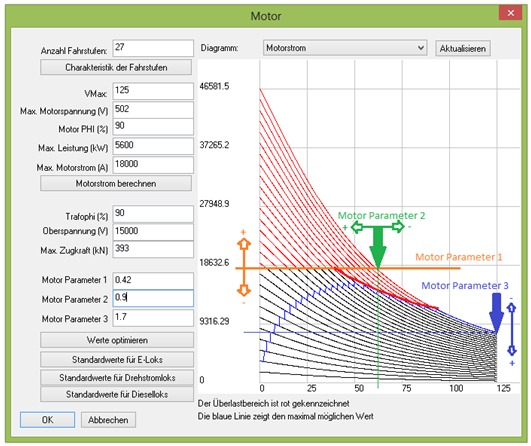
\includegraphics[width=1.0\textwidth]{editor/images/motorparameter.png}
\caption{Motorparameter der Ae 610 der SBB}
\label{fig:editor:motorparameter}
\end{figure}

\subsubsection{Motorparameter 1 (orange)}
Dient zur Festlegung der Stufe (oder Punkt zwischen zwei Stufen), bei der der maximale Motorstrom erreicht wird. (Im Beispiel unten zwischen der 10. und 11. Stufe).
Dazu ganz links bei Geschwindigkeit 0 aufsteigend die Anzahl schwarzer Linien zählen. Parameter 1 so lange verändern, bis gewünschte Stufe erreicht wird.

\subsubsection{Motorparameter 2 (grün)}
Legt fest, ab welchem Punkt der Motorstrom auf der höchsten Fahrstufe in Bezug auf eine bestimmte Geschwindigkeit zu sinken beginnt.
Durch Verändern des Parameters 2 kann der Punkt, an dem sich die waagrechte Linie des max. Motorstroms und die Linie der höchsten Stufe kreuzen, so waagrecht verschoben werden, bis die Senkrechte durch diesen Punkt unten auf der Geschwindigkeitsskala auf die gewünschte Geschwindigkeit trifft.

\subsubsection{Motorparameter 3 (blau)}
Bestimmt den Motorstrom, der bei maximaler Geschwindigkeit auf der höchsten Fahrstufe noch fließt.
Mit dem Verändern des Parameters 3 kann die Höhe des Motorstroms eingestellt werden, der bei max. Geschwindigkeit noch fliesst.

Es ist zu beachten, dass sich die Motorparameter 2 und 3 gegenseitig beeinflussen. Es ist deshalb meist nötig, den nicht veränderten Parameter etwas nachzuregeln, bis die Kennlinien mit dem Vorbild übereinstimmen.

Auf \fref{fig:editor:motorparameter} wurde die Oberstrom- (oder Primärstrom-)begrenzung durch eine rote Linie gekennzeichnet. Bei Loks, die keine Oberstrombegrenzung haben, fällt diese "Delle" weg.


\subsubsection{Werte optimieren}
Wenn detaillierte Werte einer Lok bekannt sind, kann man diese in eine Tabelle eingeben und Loksim erstellt daraus eine Widerstandskurve, indem es selbst die drei Parameter berechnet.

\subsection{Standardwerte für E-Loks, Drehstromloks und Dieselloks}
Stehen keine genauen Angaben für eine Lok zur Verfügung, kann man mit dieser Funktion die Kennlinien durch Loksim erstellen lassen. Ebenso dient sie als Ausgangsbasis und der Ersteller des Führerstandes kann durch Veränderung der Motorparameter die Kennlinien nachträglich manuell nach seinen Wünschen einstellen (siehe oben).

\subsubsection{Drehstromloks}
Der Parameter 1 hat bei diesen Loks eigentlich keine Bedeutung, denn hier wird mit dem Fahrhebel die prozentuale Zugkraft eingestellt. Die „Stufenlinien“ müssten daher eigentlich waagrecht liegen. Loksim ist aber zur Zeit noch nicht für Drehstromloks optimiert.
Immerhin kann mit dem Parameter 1 der Punkt mitbeeinflusst werden, an dem die maximale Lokleistung zur Verfügung steht (siehe auch Parameter 2).

Annäherungsweise kann der Parameter 2 so eingestellt werden, dass die maximale Leistung bei der Geschwindigkeit erreicht wird, bei der die Zugkraft zu sinken beginnt.

Ebenso kann mit dem Parameter 3 der Punkt angesteuert werden, an dem noch eine bestimmte Zugkraft bei max. Geschwindigkeit erbracht wird.

\subsubsection{Dieselloks}
Wenn es sich um Diesel-Generator-Loks handelt, kann die Lok wie eine Stufenschalterlok eingestellt werden. Die Dieselthematik ist zur Zeit im Loksim noch nicht umgesetzt.

\subsubsection{Dampfloks}
Da die Dampfloks ein sehr ähnliches Verhalten wie Stufenschalterloks haben, kann ihr Verhalten mittels der drei Parameter ziemlich vorbildlich nachgebaut werden, allerdings mit „artfremden“ Parametern (Spannung, Strom). Die Dampfthematik ist derzeit im Loksim noch nicht umgesetzt.

\subsection{Diagramm}
Mit dem Popup-Menu kann zwischen den Ansichten Leistung, Oberstrom, Motorstrom,  Motorspannung, Widerstand und Zugkraft gewählt werden.

\subsection{Bemerkung}
Die Zugkraft ist mit einem Fehler behaftet, was sich insbesondere bei Drehstromloks mit Zugfahrkrafthebeln bemerkbar macht. Das Antriebsmodell des Loksim wird derzeit überarbeitet (inklusive Bremsen) und voraussichtlich in einer der nächsten Versionen veröffentlicht.
